\documentclass[addpoints,11pt]{exam}

\usepackage{alltt}
\usepackage[margin=1in]{geometry}   % set up margins
\usepackage[T1]{fontenc}
\usepackage[usenames,dvipsnames]{xcolor}
\usepackage{enumerate}              % fancy enumerate
\usepackage{amsmath}                % used for \eqref{} in this document
\usepackage{amsthm}
\theoremstyle{definition}
\newtheorem{exmp}{Example}[section]
\usepackage{verbatim}               % useful for \begin{comment} and \end{comment}
\usepackage{eurosym}                % used for euro symbol
\usepackage{caption} 
\usepackage{graphicx}
\graphicspath{{Figures/}}
\usepackage{subcaption}
\usepackage{color}
\usepackage{float}
\usepackage{amssymb}
\usepackage{sgamevar}
\usepackage{sgame}
\usepackage[colorlinks=true]{hyperref}
\hypersetup{colorlinks=true, citecolor=ForestGreen, linkcolor=BlueViolet, urlcolor=Magenta}



%Solutions or nah (blank next two lines out for no solutions, unblank #3)
%\printanswers
%\newcommand{\dd}[1]{\par {\textbf{\textcolor{red}{#1}}}}
\newcommand{\dd}[1]{}  


\setlength\parindent{0pt}
\unframedsolutions
\SolutionEmphasis{\color{red}}
\CorrectChoiceEmphasis{\color{red}}
\renewcommand{\choicelabel}{(\alph{choice})}
\newcommand{\blank}[0]{\underline{\hspace{3cm}}}
\pointformat{\bfseries[\thepoints]}
\pointpoints{pt}{pts}
\pointsinrightmargin

\begin{document}


	\title{\textbf{Problem Set 4 \dd{Answers and Selected Solutions}} \\ \vspace{2 mm} {\large Principles of Economics}}
	\author{David A. D\'iaz}
	\date{}
	\maketitle

\subsection*{Monopolistic Competition}

\begin{questions}
	
	
	\question Which of the following conditions does NOT describe a firm in a monopolistically competitive market?
	
	\begin{choices}
		\choice It makes a product different from its competitors.
		\CorrectChoice It takes its price as given by market conditions.
		\choice It maximizes profit both in the short run and in the long run.
		\choice It has the freedom to enter or exit in the long run.
	\end{choices}
	

	\question Firms in monopolistically competitive markets are similar to monopolies in that they both \blank and are similar to firms in perfectly competitive markets in that they both \blank.
	
	\begin{choices}
		\choice make positive profits in the short and long run; are price takers
		\choice charge a price above the marginal cost; produce at the efficient scale in the long run
		\CorrectChoice are price makers; make zero economic profit in the long run
		\choice are in markets with barriers to entry; produce at the efficient quantity
	\end{choices}
	

	
	\question A monopolistically competitive firm will decrease its production if
	
	\begin{choices}
		\choice marginal revenue is less than average total cost.
		\choice price is less than marginal cost.
		\CorrectChoice marginal revenue is less than marginal cost.
		\choice price is less than average total cost.
	\end{choices}
		
	\question For a firm in a monopolistically competitive market, which of the following accurately describes the relationship between the price, average total cost, and marginal cost in the short run given that the firm is making a negative profit?
	
	\begin{choices}
		\choice $ATC = P = MC$
		\choice $ATC > P = MC$
		\choice $ATC = P > MC$
		\CorrectChoice $ATC > P > MC$
	\end{choices}
	
	\begin{solution}
		Firms in monopolistically competitive markets charge a mark-up over $MC$, so $P>MC$. If making a loss, $P<ATC$.
	\end{solution}
	
\newpage
	
	\question For a firm in a monopolistically competitive market, which of the following accurately describes the relationship between the price, average total cost, and marginal cost in the long run?
	
	\begin{choices}
		\choice $P = ATC = MC$
		\choice $P > ATC = MC$
		\CorrectChoice $P = ATC > MC$
		\choice $P > ATC > MC$
	\end{choices}
	
	\begin{solution}
		In long run, firms in monopolistically competitive markets make zero economic profit so $P=ATC$. Still charge mark-up over $MC$ so $P>MC$.
	\end{solution}
	
	\question Consider the environment faced by Sparkle, one of the many toothpaste brands in the market for toothpaste, shown in Figure \ref{fig1}.
	
	\begin{figure}[ht!]
		\centering
		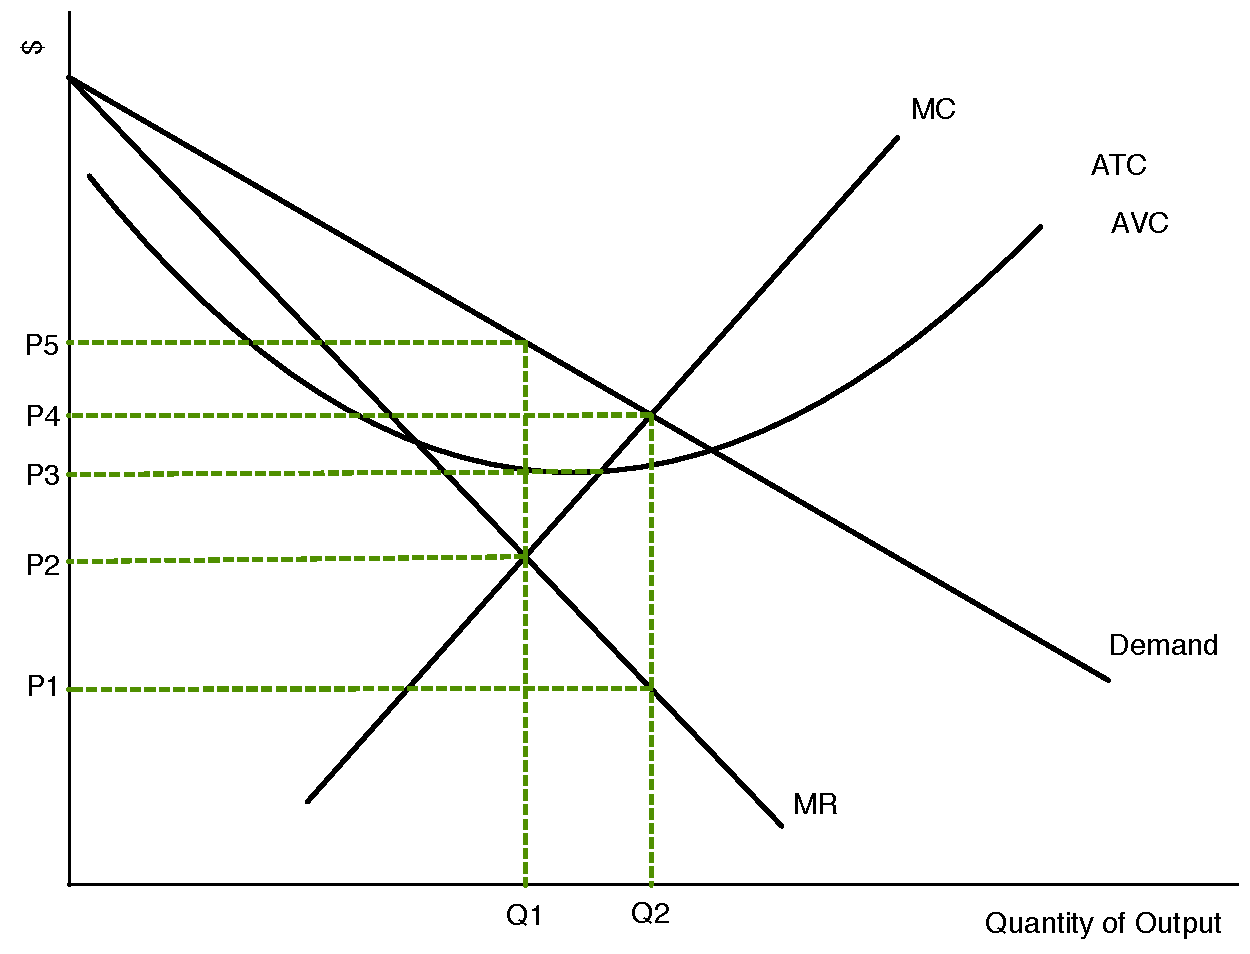
\includegraphics[scale=.40]{hw5_plot1.pdf}
		\caption{Environment for Sparkle}
		\label{fig1}
	\end{figure}
	
	The quantity produced by the firm is \underline{\hspace{3cm}} and it charges a markup of \\ \underline{\hspace{3cm}}.
	
	\begin{choices}
		\choice $Q2; P4-P3$
		\choice $Q2; P4-P1$
		\choice $Q1; P3-P2$
		\CorrectChoice $Q1; P5-P2$
	\end{choices}
	
	\begin{solution}
		Produce at $Q$ where $MR = MC$ ($Q1$). Price is point on demand curve at $Q1$ which is $P5$. Mark-up over the marginal cost = $P5 - P2$
	\end{solution}
	
\question Which of the following is true regarding the similarities and differences in monopolistic competition and monopoly?

\begin{choices}
	\choice The monopolist faces a downward-sloping demand curve while the monopolistic competitor faces a perfectly elastic demand curve.
	\CorrectChoice The monopolist makes economic profits in the long run while the monopolistic competitor makes zero economic profits in the long run.
	\choice Both the monopolist and the monopolistic competitor operate at the efficient scale.
	\choice The monopolist charges a price above marginal cost while the monopolistic competitor charges a price equal to marginal cost.
\end{choices}

\newpage

\question In the short run, if the price is above the average total cost in a monopolistically competitive market, the firm makes 

\begin{choices}
	\choice losses and firms enter the market.
	\choice losses and firms exit the market.
	\CorrectChoice profits and firms enter the market.
	\choice profits and firms exit the market.
\end{choices}

\question Monopolistically competitive firms produce 

\begin{choices}
	\choice at the efficient scale and charge a price equal to marginal cost.
	\choice at the efficient scale and charge a price above marginal cost.
	\choice with excess capacity and charge a price equal to marginal cost.
	\CorrectChoice with excess capacity and charge a price above marginal cost.
\end{choices}

\question One source of inefficiency in monopolistic competition is that

\begin{choices}
	\choice since price is above marginal cost, surplus is redistributed from buyers to sellers.
	\CorrectChoice since price is above marginal cost, some units are not produced that buyers value in excess of the cost of production.
	\choice monopolistically competitive firms produce beyond their efficient scale.
	\choice monopolistically competitive firms earn economic profits in the long run.
\end{choices}
	
	\question Sleek Sneakers Co. is one of the many firms in the market for shoes, where each company sells differentiated products.
	
	\begin{parts}
		\part Assume that Sleek is currently earning short-run profit. On a clearly labeled diagram, show the company's profit maximizing output and price, as well as the area representing profit. 
		
		\begin{solution}
			See class notes. If profit is positive, $P>ATC$ at the profit maximizing quantity, which is given by where $MR=MC$.
		\end{solution}
		
		\part What happens to Sleek's price, output, and profit in the long run? Show this in a new diagram. 
		
		\begin{solution}
			In the long run, other firms enter the market. Demand for Sleek shoes decreases and becomes more elastic. In LR, demand and ATC are tangent at the profit maximizing quantity since firms make zero economic profit. Price, output, and profit decreases.
		\end{solution}
		
		\part On your diagram for the firm in the long run, show the consumer surplus derived from the purchase of Sleek shoes and the deadweight loss relative to the efficient level of output. 
		
		\begin{solution}
			See class notes. CS is area above the price and below the demand curve. DWL comes from lost trades where demand is above $MC$.
		\end{solution}
		
		\part If the government forced Sleek to produce the efficient level of output, what would happen to the firm? 
		
		\begin{solution}
			Efficient level of output is where $P=MC$, or where demand and $MC$ intersect. But at this price, $P<ATC$ and so the firm would be making a loss.
		\end{solution}
		
	\end{parts}
	
\end{questions}

\subsection*{Oligopoly}

\begin{questions}
	
	\question If an oligopolistic industry organizes itself as a cooperative cartel, it will produce a quantity of output that is \blank the competitive level and \blank the monopoly level.
	
	\begin{choices}
		\choice less than; more than
		\choice more than; less than
		\CorrectChoice less than; equal to
		\choice equal to; more than
	\end{choices}
	
	\begin{solution}
		When acting as a cartel, firms act like a monopolist. The monopolist quantity is less than the competitive quantity.
	\end{solution}
	
\newpage
	
	\question If an oligopoly does not cooperate and each firm chooses its own quantity, the industry will produce a quantity of output that is \blank the competitive level and \blank the monopoly level.
	
	\begin{choices}
		\CorrectChoice less than; more than
		\choice more than; less than
		\choice less than; equal to
		\choice equal to; more than
	\end{choices}
	
	\begin{solution}
		Self-interest drives firms to break cartel agreement and produce more, but will still produce less than in perfect competition.
	\end{solution}
	
	
	\uplevel{For questions \ref{blah7} and \ref{blah8}, consider the simultaneous move game below.}
	
	\renewcommand{\gamestretch}{1.5}
	\sgcolsep=25pt
	\begin{figure}[htb]\hspace*{\fill}%
		\begin{game}{2}{2}[Mexico][United States] 
			&  Low tariffs & High Tariffs \\
			Low tariffs & \$25M, \$25M & \$10M, \$30M \\
			High tariffs & \$30M, \$10M & \$20M, \$20M \\
		\end{game} 
		\hspace*{\fill}%
	\end{figure}
	
	
	\question \label{blah7}The dominant strategy for Mexico is \blank and the dominant strategy for the US is \blank.
	
	\begin{choices}
		\choice low tariffs; low tariffs
		\choice high tariffs; low tariffs
		\choice low tariffs; high tariffs
		\CorrectChoice high tariffs; high tariffs
	\end{choices}
	
	\begin{solution}
		If US plays low tariffs, Mexico better of choosing high tariffs (30>25). If US plays high tariffs, Mexico still better off playing high tariffs (20>10). HT is dominant strategy for Mexico. Same for US.
	\end{solution}
	
	\item \label{blah8} Thus, the Nash Equilibrium is where the United States plays \blank and Mexico plays \blank.
	
	\begin{choices}
		\choice low tariffs; low tariffs
		\choice high tariffs; low tariffs
		\choice low tariffs; high tariffs
		\CorrectChoice high tariffs; high tariffs
	\end{choices}
	
	\begin{solution}
		Neither country can do better given the other country's strategy at (HT, HT).
	\end{solution}

	
	\question Intel and AMD each decide to either invest heavily in R\&D (``High R\&D'') or to not (``Low R\&D''). Their decisions affect both their profits and those of the other company. Assume that there is perfect information so that each knows the payoffs of the other given the strategies chosen by each. Their profits are summarized in the game table below, where the first number in each block is AMD's profit and the second number is Intel's profit.
	
	\renewcommand{\gamestretch}{1.5}
	\sgcolsep=25pt
	\begin{figure}[H]\hspace*{\fill}%
		\begin{game}{2}{2}[AMD][Intel] 
			&  High R\&D & Low R\&D \\
			High R\&D & \$15,000, \$20,000 & \$18,000, \$15,000 \\
			Low R\&D & \$16,000, \$18,000 & \$16,000, \$15,000\\
		\end{game} 
		\hspace*{\fill}%
	\end{figure}
	
\newpage
	
	If this game was played once and Intel and AMD are both rational, what would be the outcome?
	
	\begin{choices}
		\CorrectChoice Intel would invest heavily in R\&D and AMD would not.
		\choice Both Intel and AMD would invest heavily in R\&D.
		\choice AMD would invest heavily in R\&D and Intel would not.
		\choice Both Intel and AMD would choose to not invest heavily in R\&D.
	\end{choices}
	
	\begin{solution}
		AMD has no dominant strategy, but Intel has dominant strategy of high R\&D. Since AMD knows the payoffs, they know Intel has dominant strategy and that Intel will choose high R\&D. AMD's best response to this is Low R\&D. Nash eq: (low, high).
	\end{solution}
	
	\question Consider the simultaneous move game between Righty and Lefty shown below, where the first number in each block is the payoff to Lefty and the second is the payoff to Righty.
	
	\renewcommand{\gamestretch}{1.5}
	\sgcolsep=25pt
	\begin{figure}[htb]\hspace*{\fill}%
		\begin{game}{2}{2}[Lefty][Righty] 
			&  Swerve & Straight \\
			Swerve & 2, 2 & $x$, 4 \\
			Straight & 1, $y$ & 2, 3 \\
		\end{game} 
		\hspace*{\fill}%
	\end{figure}
	
	If this particular game has \textbf{no} Nash equilibrium, then possible values of $x$ and $y$ are
	
	\begin{choices}
		\choice $x=1$ and $y=2$.
		\CorrectChoice $x=1$ and $y=4$.
		\choice $x=3$ and $y=2$.
		\choice $x=3$ and $y=4$.
	\end{choices}
	
	\begin{solution}
		Lefty: If Righty chooses swerve, Lefty will choose swerve (2>1). Needs to pick Straight if Righty chooses Straight in order to not have dominant strategy $\Rightarrow x < 2.$ \\
		Righty: If Lefty chooses Swerve, Righty will choose straight (4>2). Needs to pick Swerve if Lefty chooses Straight in order to not have dominant strategy $\Rightarrow y>3.$
	\end{solution}
	
	
	
	\question Consider the simultaneous move game between Jim and Bob shown below, where the first number in each block is the payoff to Bob and the second is the payoff to Jim.
	
	\renewcommand{\gamestretch}{1.5}
	\sgcolsep=25pt
	\begin{figure}[H]\hspace*{\fill}%
		\begin{game}{2}{2}[Bob][Jim] 
			&  Left & Right \\
			Top & 2, 4 & $x$, 2 \\
			Bottom & 1, $y$ & 2, 3 \\
		\end{game} 
		\hspace*{\fill}%
	\end{figure}

	
	If ``Top'' is the dominant strategy for Bob and ``Left'' is the 	dominant strategy for Jim, then possible values of $x$ and $y$ are
	
	
	\begin{choices}
		\choice $x=1$ and $y=2$.
		\choice $x=1$ and $y=4$.
		\choice $x=3$ and $y=2$.
		\CorrectChoice $x=3$ and $y=4$.
	\end{choices}
	
	\begin{solution}
		Bob: Needs to choose Top when Jim chooses Right $\Rightarrow x>2$.\\
		Jim: Needs to choose Left when Bob chooses Bottom $\Rightarrow y>3$.
	\end{solution}
	
\newpage

	\question Bandidos and Carrburritos are the only taco sellers in Chapel Hill. They face the environment outlined in Table \ref{MC24}. 
	
	\begin{table}[H]
		\caption{Demand Schedule and Costs for Tacos in CH}
		\centering
		\begin{tabular}{c|c|c}
			Price & Quantity Demanded & Average Total Cost \\
			\hline
			\$10 & 200 & \$4\\
			\$9 & 300 & \$4\\
			\$8 & 400 & \$4 \\
			\$7 & 500 & \$4 \\
			\$6 & 600 & \$4 \\
		\end{tabular} 
		\label{MC24}
	\end{table}
	
	The two firms currently have an agreement where they produce 400 tacos in total and split production evenly. If Bandidos were to break this agreement and increased their taco production by 100 tacos while Carrburritos stuck to the original agreement, the profit realized by Bandidos would now be \underline{\hspace{3cm}} and the profit realized by Carrburritos would be \blank.
	
	
	\begin{choices}
		\CorrectChoice \$900; \$600
		\choice \$750; \$750
		\choice \$900; \$700
		\choice \$800; \$800
	\end{choices} 


\question A situation in which oligopolists interacting with one another each choose their best strategy given the strategies that all the other oligopolists have chosen is known as a 

\begin{choices}
	\choice collusions solution.
	\choice cartel.
	\CorrectChoice Nash equilibrium.
	\choice dominant strategy.
\end{choices}	

\question If oligopolists engage in collusion and successfully form a cartel, the market outcome is 

\begin{choices}
	\CorrectChoice the same as if it were served by a monopolist.
	\choice the same as if it were served by competitive firms.
	\choice efficient because cooperation improves efficiency.
	\choice known as a Nash equilbrium.
\end{choices}
	
	\question Jack and Jill are the only lemonade providers in Jurassic World. They face the environment outlined in Table \ref{MC21}. 
	
	

	\begin{table}[H]
		\caption{Demand Schedule and Costs Lemonade}
		\centering
		\begin{tabular}{c|c|c}
			Price & Quantity Demanded & Average Total Cost \\
			\hline
			\$1.10 & 300 & \$.30\\
			\$1.00 & 400 & \$.30\\
			\$.90 & 500 & \$.30\\
			\$.80 & 600 & \$.30 \\
			\$.70 & 700 & \$.30 \\
			\$.60 & 800 & \$.30 \\
		\end{tabular} 
		\label{MC21}
	\end{table}
	
	
	\begin{parts}
		
		\part The two friends currently have an agreement where they produce 600 drinks in total and split production evenly. What will be the profit realized by each individual? 
		
		\begin{solution}
			To sell 600 drinks, they will charge price of \$.80 and realize total profit of $\Pi = (.80 - .30)\times 600 = \$300$. Since they split production, profit of each will be \$150.
		\end{solution}
		
		\part If Jack were to break this agreement and increase his lemonade stand's production by 100 drinks, while Jill stuck to the original agreement, what will be the profit realized by each?
		
		\begin{solution}
			With quantity demanded of 700, price will decrease to \$.70. Jack will realize profit of $\Pi = (.70 - .30) \times 400 = \$160$, while Jill will only realize profit of $\Pi = (.70 - .30) \times 300 = \$120$.
		\end{solution}
		
		\part What will be the profit realized by each if both choose to increase production by 100 units? 
		
		\begin{solution}
			New price will be \$.60 since quantity demanded is 800. Profit for each is $\Pi = (.60 - .30) \times 400 = \$120$.
		\end{solution}
		
		
	\end{parts}
	
	
	
	\question Consider the three person simultaneous move game below. Each person can decide to either work or shirk. Alice chooses the row, Bob chooses the column, and Curt chooses the matrix. For example, if Alice decides to work, Bob decides to shirk, and Curt decides to work, the payoffs are given by the top row of the right column of the top matrix. Alice would get a payoff of $-1/2$, Bob would get a payoff of $3/2$, and Curt would get a payoff of $1$.
	
	
	\begin{center} Curt: Work \end{center}
	\renewcommand{\gamestretch}{1.5}
	\sgcolsep=25pt
	\begin{figure}[H]\hspace*{\fill}%
		\begin{game}{2}{2}[Alice][Bob] 
			&  Work & Shirk \\
			Work & 1, 1, 1 & $-1/2$, $3/2$, 1 \\
			Shirk & $3/2$, 1, $-1/2$ & 0, $3/2$, $-1/2$ \\
		\end{game} 
		\hspace*{\fill}%
	\end{figure}
	
	\begin{center} Curt: Shirk \end{center}
	\renewcommand{\gamestretch}{1.5}
	\sgcolsep=25pt
	\begin{figure}[htb]\hspace*{\fill}%
		\begin{game}{2}{2}[Alice][Bob] 
			&  Work & Shirk \\
			Work & 1, $-1/2$, 3/2 & $-1/2$, 0, 3/2 \\
			Shirk & $3/2$, $-1/2$, 0 & 0, 0, 0 \\
		\end{game} 
		\hspace*{\fill}%
	\end{figure}
	
	
	\begin{parts}
		\part Does Alice have a dominant strategy? If so, what is it? 
		
		\begin{solution}Top matrix: Curt chooses work. If Bob works, Alice better off shirking (3/2>1). If Bob shirks, Alice is better off shirking (0>--1/2). \\
			Bottom matrix: Curt chooses shirk. If Bob works, Alice is better off shirking (3/2>1). If Bob shirks, Alice is better off shirking (0>--1/2). \\
			Since Alice is better off shirking regardless of the other players' strategies, her dominant strategy is to shirk.
		\end{solution}
		
		\part Does Bob have a dominant strategy? If so, what is it?
		
		\begin{solution}
			Similar analysis to (a). Dominant strategy is to shirk.
		\end{solution}
		
		\part Does Curt have a dominant strategy? If so, what is it? 
		\begin{solution}
			A little trickier, as you have to compare entries across the matrices. For example, if Alice and Bob both work, Curt's payoffs are either 1 if he works (3rd entry of top left corner of top matrix) or 3/2 (3rd entry of top left corner of bottom matrix). Continuing this way for each Alice and Bob strategy combination, Curt's dominant strategy is also to shirk.
		\end{solution}
		
		\part If there is one, what is the Nash equilibrium in this game? 
		\begin{solution}
			Nash eq. is (shirk, shirk, shirk). Payoff are given by bottom right corner of the bottom matrix.
		\end{solution}
	\end{parts}
	
\end{questions}

\subsection*{Gross Domestic Product}

\begin{questions}

		\question Which of the following does NOT add to US GDP?
		
		\begin{choices}
			\choice Air France buys a plane from Boeing, the US aircraft manufacturer.
			\choice General Motors builds a new factory in North Carolina.
			\choice The city of New York pays a salary to a policeman.
			\CorrectChoice The federal government sends a social security check to your grandmother.
		\end{choices}
		
		\begin{solution}
			Transfer payments are not included in GDP.
		\end{solution}
	
\newpage
		
		\question Which of the following is NOT considered an investment for calculating GDP?
		
		\begin{choices}
			\choice A family purchases a new home.
			\CorrectChoice An investor purchases Apple stock.
			\choice A farmer buys a new tractor.
			\choice KIA Motors builds a new factory.
		\end{choices}
		
		\begin{solution}
			Investment includes spending on capital equipment and purchases of new housing, but financial market transactions are not included in GDP because they do not represent real production.
		\end{solution}
		
		\question A country experiencing low GDP growth and high population growth will have a
		
		\begin{choices}
			\choice low real GDP growth rate.
			\choice low nominal GDP growth rate.
			\CorrectChoice low per capita GDP growth rate.
			\choice high per capita GDP growth rate.
		\end{choices}
		
		\begin{solution}
			$\hat{y} \approx \hat{Y} - \hat{N}$. Low GDP growth and high population growth will lead to low per capita GDP growth.
		\end{solution}

	\question A country experiencing high GDP growth and low population growth will have a
	
	\begin{choices}
		\choice low real GDP growth rate.
		\choice low nominal GDP growth rate.
		\choice low per capita GDP growth rate.
		\CorrectChoice high per capita GDP growth rate.
	\end{choices}
	
		\begin{solution}
			See \#3.
		\end{solution}
		
\question A bag of sugar is sold to Coca Cola for \$0.50, which uses this sugar to make Sprite that is sold to consumers for \$1.25. Another bag of of sugar is sold to Food Lion for \$1.25, where it is sold to consumers for \$2.75. Together, these transactions have what effect on GDP?


\begin{choices}
	\choice Increase GDP by \$1.75
	\CorrectChoice Increase GDP by \$4.00
	\choice Increase GDP by \$5.75
	\choice Increase GDP by \$3.00
\end{choices}
		
		\question An American buys a pair of shoes manufactured in Italy. How do the US national income accounts treat this transaction?
		
		\begin{choices}
			\choice Net exports and GDP both rise.
			\choice Net exports and GDP both fall.
			\CorrectChoice Net exports fall, while GDP is unchanged.
			\choice Net exports are unchanged, while GDP rises.
		\end{choices}
		
		\begin{solution}
			Consumption increases, while imports rises. $NX$ falls. The increase in $C$ is offset by the fall in $NX$ and $Y$ is unaffected.
		\end{solution}
		
		\question If nominal GDP rose in 2008, then we can conclude that 
		
		\begin{choices}
			\choice production rose in 2008.
			\choice prices rose in 2008.
			\choice neither production or prices rose in 2008.
			\CorrectChoice either production or prices, or both, rose in 2008.
		\end{choices}
		
		\begin{solution}
			Nominal GDP is given by current year production and current year prices, so increases in nominal GDP can be due to either.
		\end{solution}
		
\newpage
		
		\question Table \ref{MC23} shows the prices and quantities produced of the only two goods in Uzbeki-beki-beki-Stan-Stan, grapes and olives, for the years 2000 -- 2002.
		
		\begin{table}[H]
			\caption{Grapes and Olives in UZN}
			\centering
			\begin{tabular}{c|c|c|c|c}
				Year & Grapes Produced & Price of Grapes & Olives Produced & Price of Olives \\
				\hline
				2000 & 20 & \$2.10 & 4 & \$4.10\\
				2001 & 19 & \$2.25 & 6 & \$4.15\\
				2002 & 22 & \$2.20 & 7 & \$4.15\\
			\end{tabular} 
			\label{MC23}
		\end{table}
		
			Using 2001 as the base year, the real GDP in 2000 is \blank. Additionally, the inflation rate in 2001 was \blank.
			
			\begin{choices}
				\choice \$61.60; 3.2\%
				\choice \$58.4; 5.5\%
				\CorrectChoice \$61.60; 5.5\%
				\choice \$58.4; 3.2\%
			\end{choices}
			
			\begin{solution}
				Real GDP 2000 = $20 \times \$2.25 + 4 \times \$4.15 = \$61.60$ (2000 production and 2001 prices). \\
				Nominal GDP 2000 = $20 \times \$2.10 + 4\times \$4.10 = \$58.4$. \\ GDP deflator (2000) = $(58.4/61)\times 100 = 94.8$. \\
				GDP deflator (2001) = 100 (base yr.) \\
				$\pi_{2001} = (100-94.8)/94.8\times 100\% = 5.5\%$.
			\end{solution}
			
\question Which of the following would be excluded from 2016 GDP? The sale of 

\begin{choices}
	\choice a 2016 Honda made in South Carolina.
	\choice a haircut.
	\choice a realtor's services.
	\CorrectChoice a home built in 2015 and first sold in 2016.
	\choice All of the above should be included in 2016 GDP.
\end{choices}

\question GDP would include which of the following?

\begin{choices}
	\choice Housework.
	\choice Illegal drug sales.
	\choice Intermediate sales.
	\CorrectChoice Consulting services.
	\choice The value of taking a day off work.
\end{choices}

\question GDP would exclude which of the following?

\begin{choices}
	\choice Lawyer services purchased by a home buyer.
	\choice Lawn care services purchased by a home owner.
	\choice A new bridge purchased by the state of Ohio.
	\CorrectChoice Cotton purchased by Levi's Jeans.
	\choice The purchase of a new Mazda produced in Detroit.
\end{choices}

\question An example of a transfer payment is 

\begin{choices}
	\choice your employer directly depositing wages in your bank account.
	\choice remittance payments from migrants to families in their native country.
	\choice your local government paying for park maintenance.
	\CorrectChoice your state government paying unemployment benefits.
\end{choices}
			
		\question Table \ref{tab1} shows some data from the land of milk and honey. 
		
		\begin{table}[H]
			\centering
			\caption{Land of Milk and Honey}
			\label{tab1}
			\begin{tabular}{  c| c | c | c |c}        
				
				Year & Price of Milk & Quantity of Milk & Price of Honey & Quantity of Honey   \\
				\hline
				2013 & \$1 & 100 quarts & \$2 & 50 quarts \\
				2014 & \$1 & 200 & \$2 & 100 \\
				2015 & \$2 & 200 & \$4 & 100 \\
			\end{tabular}
		\end{table} 
		
		\begin{parts}
			\part Compute the nominal and real GDP for each year, using 2013 as the base year. 
			
			\begin{solution}
				Nominal GDP$_t$ = $\sum P_t \cdot Q_t$, real GDP$_t = \sum P_{base yr.}\cdot Q_t$. \\
				2013: $Y^N$ = \$1(100) + \$2(50) = \$200. $Y^R$ = \$1(100) + \$2(50) = \$200.\\
				2014: $Y^N$ = \$1(200) + \$2(100) = \$400. $Y^R$ = \$1(200) + \$2(100) = \$400. \\
				2015: $Y^N$ = \$2(200) + \$4(100) = \$800. $Y^R$ = \$1(200) + \$2(100) = \$400.
			\end{solution}
			
			\part Compute the percentage change in nominal and real GDP in 2014 and 2015. 
			
			\begin{solution}
				$\widehat{Y^N}_{2014} = (400 - 200)/200 = 100\%$. $\widehat{Y^N}_{2015} = (800-400)/400 = 100\%$. \\
				$\widehat{Y^R}_{2014} = (400 - 200)/200 = 100\%$. $\widehat{Y^R}_{2015} = (400-400)/400 = 0\%$.
			\end{solution}
			
			\part Did economic well-being rise more in 2014 or 2015? Explain. 
			
			\begin{solution}
				Real GDP is a better measure of economic well-being. It increased by more in 2014, so well-being rose more in 2014.
			\end{solution}
		\end{parts}		
	
\end{questions}

\subsection*{Measuring the Cost of Living}

\begin{questions}

			\question If the consumer price index was 200 in 1980 and 300 today, then \$600 in 1980 would have the same purchasing power as \blank today.
			
			\begin{choices}
				\choice \$400
				\choice \$500
				\choice \$700
				\CorrectChoice \$900
			\end{choices}
			
		\begin{solution}
			Amount in 2016 dollars = amount in 1980 dollars $\times (CPI_{2016}/CPI_{1980})$ = \$600 $\times$ (300/200) = \$900.
		\end{solution}

		\question Suppose the CPI in 1990 using 1980 as the base year was 114, while the CPI in 1980 using 1975 as the base year was 105. If average salary of engineers in 1990 was \$74,500 and they were equally as well off in terms of purchasing power as engineers were in 1980, then the average salary of engineers in 1980 must have been approximately
		
		\begin{choices}
			\CorrectChoice \$65,351.
			\choice \$84,930.
			\choice \$74,500.
			\choice \$68,618.
		\end{choices}
		
		\begin{solution}
			CPI 1990 (1980 base year) = 114. \\
			CPI 1980 (1980 base year) = 100. \\
			1980 salary in 1990 dollars = 1980 salary $\times (CPI_{1990}/CPI_{1980})$ = 1980 salary $\times (114/100) = \$74,500 \Rightarrow$ 1980 salary = \$65,351. 
		\end{solution}
		

	\question Assume an economy experienced a positive rate of inflation between 2003 and 2004 and again between 2004 and 2005. However, the inflation rate was lower between 2004 and 2005 than it was between 2003 and 2004. Which of the following scenarios is consistent with this assumption?
	
	
	
	\begin{choices}
		\choice The CPI was 100 in 2003, 110 in 2004, and 105 in 2005.
		\CorrectChoice The CPI was 100 in 2003, 120 in 2004, and 135 in 2005.
		\choice The CPI was 110 in 2003, 106 in 2004, and 100 in 2005.
		\choice All of the above are correct.
	\end{choices}
			
		\question You deposit \$2,000 in a savings account, and a year later you have \$2,100. Meanwhile, the CPI rose from 200 to 204. In this case, the nominal interest rate is \blank and the real interest rate is \blank.
		
			
			\begin{choices}
				\choice 1\%; 5\% 
				\choice 3\%; 5\%
				\choice 5\%; 1\%
				\CorrectChoice 5\%; 3\%
			\end{choices}
			
			\begin{solution}
				Nominal interest rate = $(2100-2000)/2000 = 5\%.$ Inflation = $(204-200)/200 = 2\%$. Real interest rate = nominal interest rate - inflation = 3\%.
			\end{solution}
			
			\question When the consumer price index rises, the typical family
			
			\begin{choices}
				\CorrectChoice has to spend more dollars to maintain the same standard of living.
				\choice can spend fewer dollars to maintain the same standard of living.
				\choice finds that its standard of living is not affected.
				\choice can offset the effects of rising prices by saving more.
			\end{choices}
			
		\begin{solution}
			As the CPI increases so do the costs of living. Thus, have to spend more dollars in order to maintain an equivalent standard.
		\end{solution}
				
			\question One of the widely-acknowledged problems with the consumer price index (CPI) as a measure of the cost of living is that the CPI
					
					
					\begin{choices}
						\choice fails to account for consumer spending on housing.
						\choice accounts only for consumer spending on food, clothing, and energy.
						\choice fails to account for the fact that consumers spend larger percentages of their incomes on some goods and smaller percentages of their incomes on other goods.
						\CorrectChoice fails to account for the introduction of new goods.
					\end{choices}
					
			
				
				
			\question Suppose the CPI in 2001 using 1982 as the base year was 262. The average salary of accounting majors in 1982 was \$45,500, while in 2001 it was \$74,000. Given this information, we can say that accounting majors in 2001 were
			
			\begin{choices}
				\choice better off than accounting majors in 1982.
				\CorrectChoice worse off than accounting majors in 1982.
				\choice equally as well off as accounting majors in 1982.
				\choice Not enough information given.
			\end{choices}
			
			\begin{solution}
				2001 dollars in 1982 dollars = 74,000 $\times$ 100/262 = \$28,244 (CPI in 1982 = 100 since it is the base year). Since this is less than how much accountants made in 1982, accountants in 2001 are worse off. \\
				Could also calculate 1982 salary in 2001 dollars = 45,500 $\times$ 262/100 = \$119,210 to see that accounts are worse off.
			\end{solution}
		
			\question Mavis Corporation has an agreement with its workers to index completely the wage of its employees to the CPI. Mavis currently pays its production line workers \$7.50 an hour and is scheduled to index their wages today. If the CPI is currently about 130 and was 120 a year ago, Mavis should increase the hourly wages of its workers by about
			
			\begin{choices}
				\choice \$0.075
				\choice  \$0.10.
				\choice \$0.58.
				\CorrectChoice \$0.63.
			\end{choices}
			
			\begin{solution}
				Inflation was (130 - 120)/120 = 8.33\%, so new wages would have to increase by \$7.50$\times$.833 $\approx$ \$.63.
			\end{solution}
			
			
			\question The cost of a basket of goods and services in 1990 was computed to be \$90. In 2000, this same basket's cost was computed to be \$85. Moreover, the CPI in 2001 using 1990 as the base year was 90. What was the inflation rate between 2000 and 2001?
			
			\begin{choices}
				\choice $-5.88\%$
				\choice 4.70\%
				\CorrectChoice $-4.70\%$
				\choice 5.88\%
			\end{choices}
			
			\begin{solution}
				CPI in 2000 using 1990 as base year = (85/90)$\times$100 = 94.44. Inflation between 2000 and 2001 = (90-94.44)/94.44 = --4.70\%.
			\end{solution}

\newpage

\question The ``basket'' on which the CPI is based is composed of 

\begin{choices}
	\choice raw materials purchased by firms.
	\choice total current production.
	\CorrectChoice products purchased by the typical consumer.
	\choice consumer production.
	\choice none of the above.
\end{choices}


\question Suppose your income rises from \$19,000 to \$31,000 while the CPI rises from 122 to 169. Your standard of living has likely

\begin{choices}
	\choice fallen.
	\CorrectChoice risen.
	\choice stayed the same.
	\choice Impossible to tell without knowing the base year.
\end{choices}

\question If workers and firms agree on an increase in wages based on their expectations of inflation and inflation turns out to be more than expected,

\begin{choices}
	\CorrectChoice firms will gain at the expense of workers.
	\choice workers will gain at the expense of firms.
	\choice neither firms nor workers will gain because the increase in wages is fixed in the labor agreement.
	\choice both firms and workers will gain because the increase in wages is fixed in the labor agreement.
\end{choices}
			
		\question Table \ref{tab2} refers to a small economy that produces two goods - books and calculators. A typical basket of books and calculators consists of 10 books and 2 calculators.
		
		\begin{table}[H]
			\caption{Books and Calculators}
			\label{tab2}
			\centering
			\begin{tabular}{  c|c|c}        
				
				Year   & Price of Books & Price of Calculators \\
				\hline
				2010 &  \$30 & \$4.00\\
				2011 & \$35 & \$4.50\\
				2012 & \$35 & \$6.00 \\
			\end{tabular}
		\end{table}
		\begin{parts}
			\part Calculate the consumer price index for each year, using 2012 as the base year. 
			
			\begin{solution}
				Basket: 10 books, 2 calculators remains fixed. \\
				$P_{2010} = 10\times \$30 + 2\times \$4 = \$308$\\
				$P_{2011} = 10\times \$35 + 2\times \$4.50 = \$359$ \\
				$P_{2012} = 10\times \$35 + 2\times \$6 = \$362$ \\
				CPI$_t$ = $P_t/P_{base yr.}\times 100$. \\
				CPI$_{2010} = (308/362)\times 100 = 85.1$ \\
				CPI$_{2011} = (359/362)\times 100 = 99.2$ \\
				CPI$_{2012} = (362/362)\times 100 = 85.1$ 
			\end{solution}
			
			\part Calculate the inflation rate for 2011 and 2012. 
			
			\begin{solution}
				$\pi_{2011} = (99.2-85.1)/85.1 = 16.57\%.$ \\
				$\pi_{2012} = (100-99.2)/99.2 = .81\%.$ 
			\end{solution}
			
			\part The average salary of a plumber in 2010 was \$22,500, while in 2012 the average salary was \$24,975. Were plumbers better off in 2012 relative to 2010? Explain why. 
			
			\begin{solution}
				2010 salary in 2012 dollars = \$22,500 $\times$ (100/85.1) = \$26,439.48. Plumbers were better off in 2010 (salaries increased by 11\%, but prices increased by approximately 17\% $\Rightarrow$ purchasing power decreased.)
			\end{solution}
			
		\end{parts}
			
\end{questions}


\end{document}